\documentclass[12pt, a4paper]{extarticle}
\usepackage{amsfonts}
\usepackage{listings}
\usepackage{amsthm}
%\usepackage[T2A]{fontenc}
\usepackage[utf8]{inputenc}
%\usepackage{mathtext}  
\usepackage{amsmath, amsfonts, amssymb}
\usepackage[russian]{babel}
\usepackage[body={17.5cm, 23.5cm},left=3cm, top=2cm, right=2cm, bottom=2cm]{geometry}
\usepackage{graphicx}
\graphicspath{{pictures/}}
\DeclareGraphicsExtensions{.pdf,.png,.jpg}
\usepackage{blindtext}
\usepackage{fancyhdr}
\usepackage{graphicx}
\usepackage{ragged2e}
\usepackage{misccorr} % в заголовках появляется точка, но при ссылке на них ее нет 
\usepackage{indentfirst} % после заголовков ставится абзацный отступ
%\parindent{1.25cm} 
\newcommand{\specialcell}[2][c]{%
  \begin{tabular}[#1]{@{}c@{}}#2\end{tabular}}
\graphicspath{images/}
\setcounter{tocdepth}{6}
\newtheorem{theorem}{Теорема}
\newcommand{\eps}{\varepsilon}
\newcommand{\re}{\operatorname{Re}}
\newcommand{\im}{\operatorname{Im}}
\renewcommand{\labelitemi}{$-$}
\renewenvironment{itemize}[1][{---\hfil}]{\begin{list}{#1}{\topsep=0pt\parsep=0pt plus 1pt\itemsep=\parsep\leftmargin=0pt \itemindent=\parindent}\addtolength{\itemindent}{\labelwidth}}{\end{list}}
%\setcounter{page}{}
\begin{document}
Из (15) следует, что  $A=-C$   и $B= -D $. В результате имеем для системы (15)-(17) матрицу, определитель которой определяет  характеристическое уравнение $P(\beta)=0$, которое,в свою очередь, определяет собственные значения $\beta_j> 0 (\lambda_j=\beta^4_j)$
			\begin{equation*}
			\begin{pmatrix}
			A_{11}& A_{12} \\
			A_{21} & A_{22}
			\end{pmatrix} 
			\end{equation*}
			\begin{multline*}			
			A_{11}=-\beta^2(\cosh(\beta)+\cos(\beta))+\lambda M J \beta(\sinh(\beta)+ \sin(\beta))+ a \lambda M(\cosh(\beta)-\\-ac(\cosh(\beta)-\cos(\beta))-a^2 c \beta(\sinh(\beta)+\sin(\beta)) 
			\\ 
			A_{12}= -\beta^2(\sinh(\beta)+ \sin(\beta))+\lambda M J \beta(\cosh(\beta)-\cos(\beta))+ a \lambda M(\sinh(\beta)- \sin(\beta))-\\-ac(\sinh(\beta)- \sin(\beta))-a^2 c \beta(\cosh(\beta)-\cos(\beta))  
			\\
			A_{21}=-\beta^3(\sinh(\beta)+ \sin(\beta)) - (\lambda M-c) (\cosh(\beta)-\cos(\beta)) - (\lambda M-c) a \beta(\sinh(\beta)+ \sin(\beta)) 
			\\
			A_{22}=-\beta^3(\cosh(\beta)+\cos(\beta))
			 -(\lambda M-c) (\sinh(\beta)- \sin(\beta))  - (\lambda M-c) a \beta(\cosh(\beta)-\cos(\beta))			
			\end{multline*}
			\begin{equation*}
			P(\beta)=A_{11} A_{12}-A_{21} A_{22}=0
			\end{equation*}
			В ходе выполнения работы была написана программа на языке Python, вычисляющая первые 5 положительных корней характеристического уравнения, и строящая соответствующие им собственные функции $\nu_j(x)$
			\begin{figure}[h!]
             \centering
              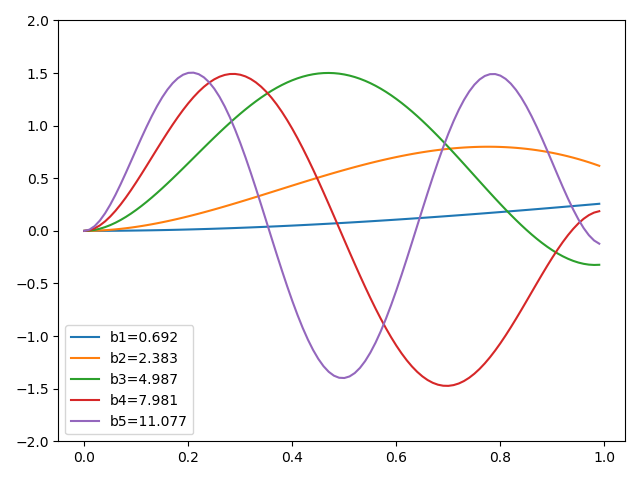
\includegraphics[scale=0.6]{EigenFunc(c=0.1)}
              \caption{$c=0.1, d=0.025, l=0.5, d_1=0.08, l_1=0.3$}
			\end{figure}
			\begin{figure}[h!]
             \centering
              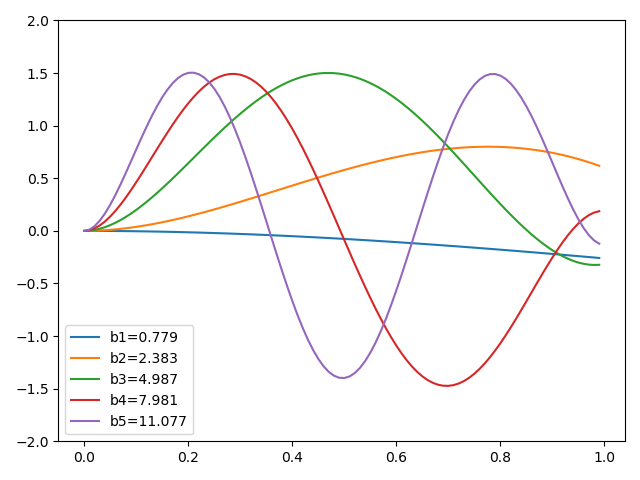
\includegraphics[scale=0.6]{EigenFunc(c=1)}
              \caption{$c=1, d=0.025, l=0.5, d_1=0.08, l_1=0.3$}
			\end{figure}
			\newpage
			\begin{figure}[h!]
             \centering
              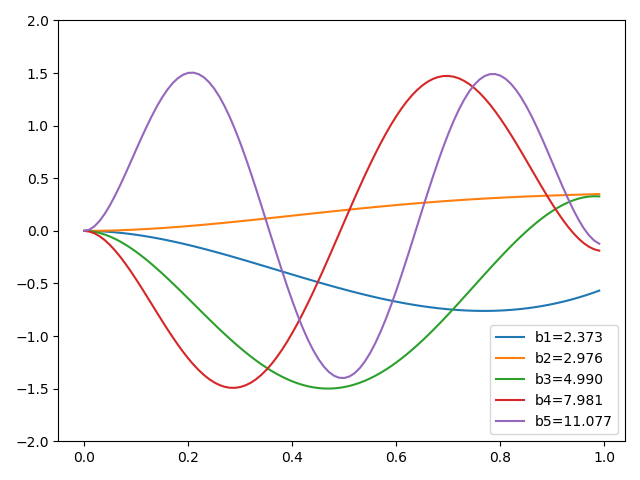
\includegraphics[scale=0.6]{EigenFunc(c=500)}
              \caption{$c=500, d=0.025, l=0.5, d_1=0.08, l_1=0.3$}
			\end{figure}
			\begin{figure}[h!]
             \centering
              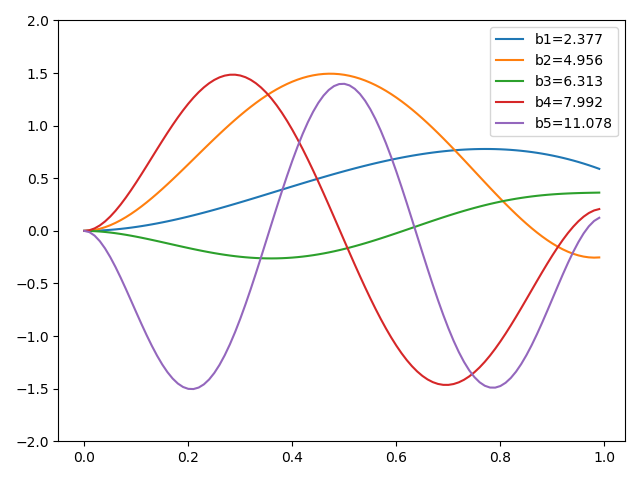
\includegraphics[scale=0.6]{EigenFunc(c=10000)}
              \caption{$c=10000, d=0.025, l=0.5, d_1=0.08, l_1=0.3$}
			\end{figure}
			\newpage
			Собственные функции удовлетворяют следующим условиям нормировки
			\begin{equation*}
			\left<\upsilon,\nu \right>=\int\limits_0^1 \upsilon(x) \nu(x) dx +M\upsilon(1)\nu(1) + M J \upsilon'(1)\nu'(1) + M a (\upsilon'(1)\nu(1)+\upsilon(1)\nu'(1))
			\end{equation*}
			\begin{equation*}
			\|\upsilon\|=\left<\upsilon, \upsilon \right>^{1/2}
			\end{equation*}
				\newpage
				По теорме о неявной функции имеем для $\lambda_{*1}$:
$$\lambda_{*1} = - \frac {f_{\epsilon}(i\sigma_{1*}; 0)}{f_{\lambda}(i\sigma_{1*}; 0)} = - \frac{a_{0*} i \sigma_{1*}}{2 i \sigma_{1*} + a_{0*}} = - \frac{a_{0*} i \sigma_{1*} + 2 \sigma_{1*}^2 a_{0*}}{a_{0*} + 4 \sigma_{1*}}$$

Вещественная часть $\lambda_{*1} = -\frac{2 \sigma_{1*}^2 a_{0*}}{a_{0*} + 4\sigma_{1*}^2}$ < 0, следовательно, при увеличении параметра $a_{0}$ нули характеристического уравнения с мнимой оси переходят в $\mathbb {C}_{-}$. На основании этим данных строим картину $D$-разбиений, где $D_{j}$ обозначает область, где характеристическое уравнение имеет j нулей, принадлежащих полуплоскости $\mathbb {C}_{+}$.
\\
\begin{figure}[h!]
 \centering
 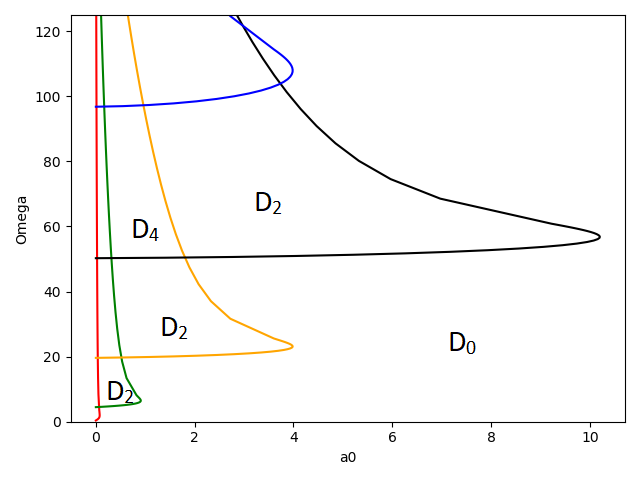
\includegraphics[scale=0.8]{D-razb_c=0.1}
 \caption{$c=0.1, d=0.025, l=0.5, d_1=0.08, l_1=0.3$}
\end{figure}
\begin{figure}[h!]
 \centering
 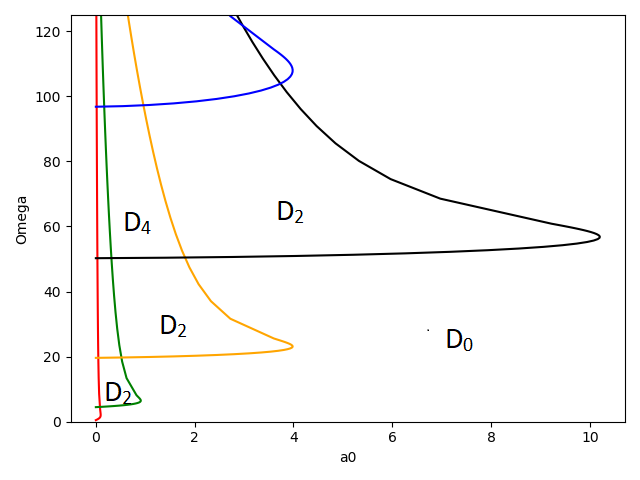
\includegraphics[scale=0.8]{D-razb_c=1}
 \caption{$c=1, d=0.025, l=0.5, d_1=0.08, l_1=0.3$}
\end{figure}
\begin{figure}[h!]
 \centering
 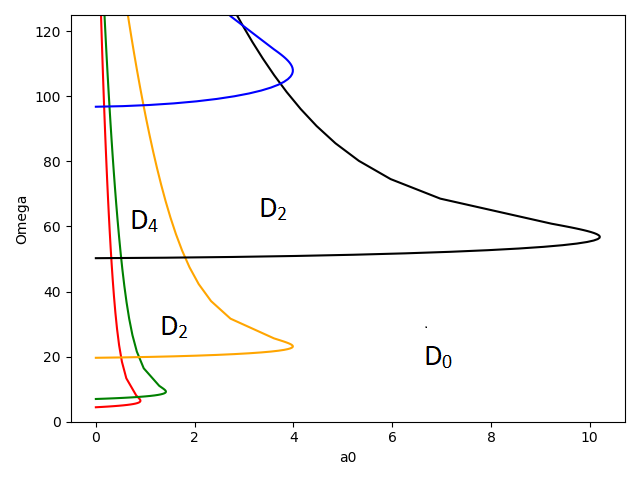
\includegraphics[scale=0.8]{D-razb_c=500}
 \caption{$c=500, d=0.025, l=0.5, d_1=0.08, l_1=0.3$}
\end{figure}
\begin{figure}[h!]
 \centering
 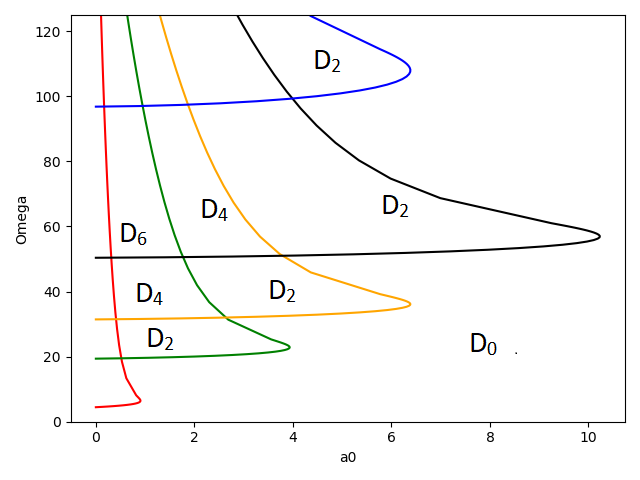
\includegraphics[scale=0.8]{D-razb_c=10000}
 \caption{$c=10000, d=0.025, l=0.5, d_1=0.08, l_1=0.3$}
\end{figure}


\newpage
\end{document}